\documentclass[tikz,border=3pt]{standalone}
\usepackage{amsmath,amssymb}
\usepackage{helvet}\renewcommand{\familydefault}{\sfdefault}
\usetikzlibrary{positioning,arrows.meta,fit,calc,decorations.pathreplacing}
\definecolor{lex}{HTML}{4C72B0}\definecolor{boi}{HTML}{DD8452}\definecolor{met}{HTML}{55A868}
\definecolor{cod}{HTML}{8172B3}\definecolor{str}{HTML}{937860}\definecolor{rep}{HTML}{C44E52}
\definecolor{edge}{HTML}{B22222}
\begin{document}
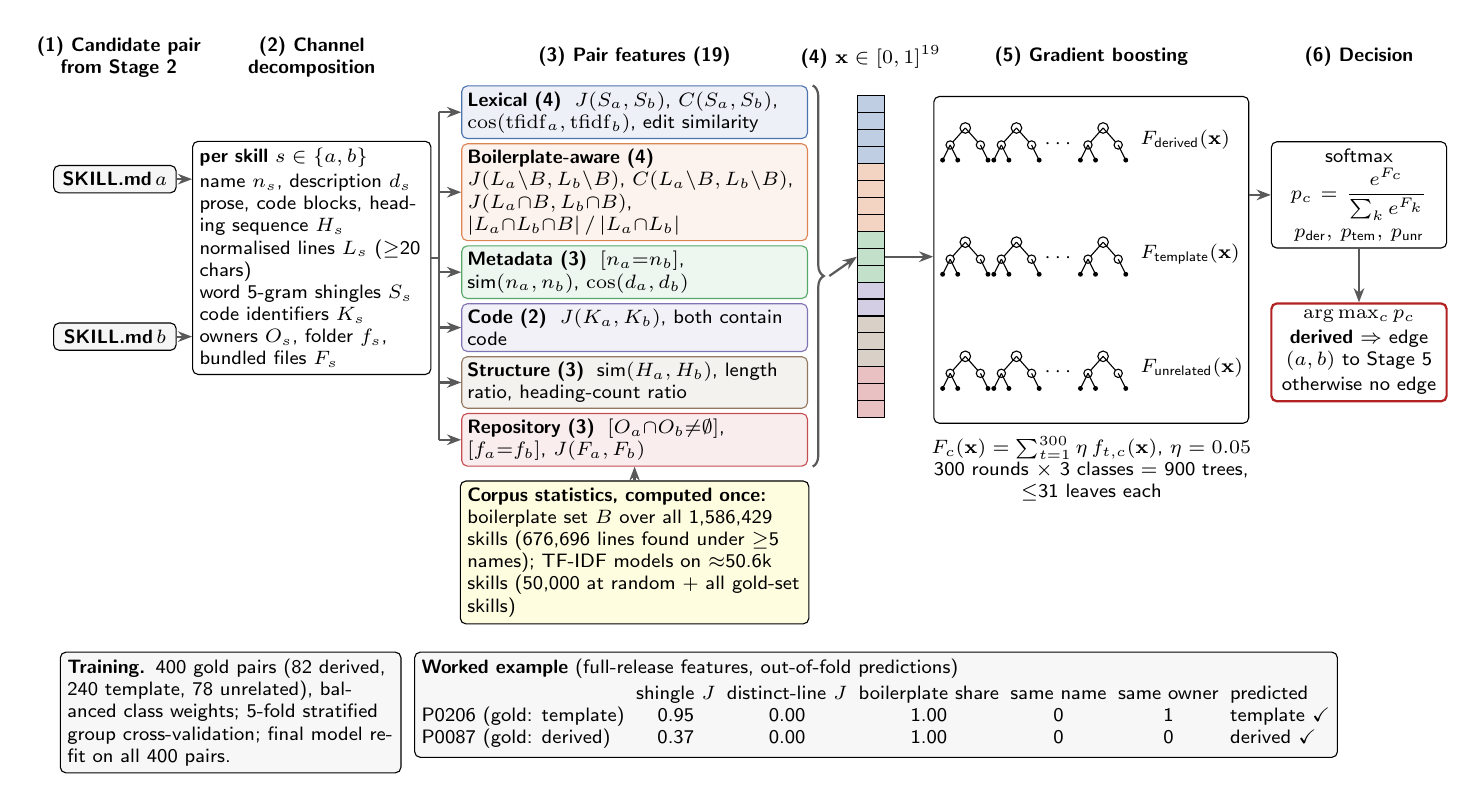
\begin{tikzpicture}[font=\scriptsize, >={Stealth[length=1.8mm]},
  box/.style={draw, rounded corners=2pt, align=left, inner sep=2.5pt},
  grp/.style={draw=#1, fill=#1!10, rounded corners=2pt, align=left, inner sep=2pt, text width=4.25cm},
  lbl/.style={font=\scriptsize\bfseries, align=center},
  flow/.style={->, thick, gray!70!black}]

% (1) input pair
\node[box, text width=1.38cm, align=center, fill=gray!8] (a) at (-0.05,1.0) {\textbf{SKILL.md}\,$a$};
\node[box, text width=1.38cm, align=center, fill=gray!8] (b) at (-0.05,-1.0) {\textbf{SKILL.md}\,$b$};
\node[lbl] at (0,2.55) {(1) Candidate pair\\from Stage 2};

% (2) channels
\node[box, text width=2.85cm] (ch) at (2.45,0) {%
\textbf{per skill $s\in\{a,b\}$}\\[1pt]
name $n_s$, description $d_s$\\
prose, code blocks, heading sequence $H_s$\\
normalised lines $L_s$ ($\geq$20 chars)\\
word 5-gram shingles $S_s$\\
code identifiers $K_s$\\
owners $O_s$, folder $f_s$, bundled files $F_s$};
\node[lbl] at (2.45,2.55) {(2) Channel\\decomposition};
\draw[flow] (a.east) -- (ch.west |- a.east);
\draw[flow] (b.east) -- (ch.west |- b.east);

% (3) feature groups
\node[grp=lex] (g1) at (6.55,1.85) {\textbf{Lexical (4)}\; $J(S_a,S_b)$, $C(S_a,S_b)$, $\cos(\mathrm{tfidf}_a,\mathrm{tfidf}_b)$, edit similarity};
\node[grp=boi, below=1.5pt of g1] (g2) {\textbf{Boilerplate-aware (4)}\; $J(L_a{\setminus}B, L_b{\setminus}B)$, $C(L_a{\setminus}B, L_b{\setminus}B)$, $J(L_a{\cap}B, L_b{\cap}B)$, $|L_a{\cap}L_b{\cap}B|\,/\,|L_a{\cap}L_b|$};
\node[grp=met, below=1.5pt of g2] (g3) {\textbf{Metadata (3)}\; $[n_a{=}n_b]$, sim$(n_a,n_b)$, $\cos(d_a,d_b)$};
\node[grp=cod, below=1.5pt of g3] (g4) {\textbf{Code (2)}\; $J(K_a,K_b)$, both contain code};
\node[grp=str, below=1.5pt of g4] (g5) {\textbf{Structure (3)}\; sim$(H_a,H_b)$, length ratio, heading-count ratio};
\node[grp=rep, below=1.5pt of g5] (g6) {\textbf{Repository (3)}\; $[O_a{\cap}O_b{\neq}\emptyset]$, $[f_a{=}f_b]$, $J(F_a,F_b)$};
\node[lbl] at (6.55,2.55) {(3) Pair features (19)};
% one bus from the channels into every group
\coordinate (bus) at ($(g1.west)+(-0.28,0)$);
\draw[thick, gray!70!black] (ch.east) -- (ch.east -| bus);
\draw[thick, gray!70!black] (bus |- g1.west) -- (bus |- g6.west);
\foreach \g in {g1,g2,g3,g4,g5,g6} \draw[flow] (bus |- \g.west) -- (\g.west);
% corpus statistics
\node[box, fill=yellow!12, text width=4.25cm, below=5pt of g6] (corp) {%
\textbf{Corpus statistics, computed once:} boilerplate set $B$ over all 1,586,429 skills (676,696 lines found under $\geq$5 names); TF-IDF models on $\approx$50.6k skills (50,000 at random + all gold-set skills)};
\draw[flow, dashed] (corp.north) -- (g6.south);

% (4) feature vector, fed by a bracket over all six groups
\foreach \k in {0,...,18} {
  \pgfmathsetmacro{\yy}{1.95-\k*0.215}
  \ifnum\k<4 \def\cc{lex}\else\ifnum\k<8 \def\cc{boi}\else\ifnum\k<11 \def\cc{met}\else\ifnum\k<13 \def\cc{cod}\else\ifnum\k<16 \def\cc{str}\else\def\cc{rep}\fi\fi\fi\fi\fi
  \node[draw, fill=\cc!35, minimum width=0.34cm, minimum height=0.215cm, inner sep=0] (v\k) at (9.55,\yy) {};
}
\node[lbl] at (9.55,2.55) {(4) $\mathbf{x}\in[0,1]^{19}$};
\draw[decorate, decoration={brace, amplitude=4pt}, thick, gray!70!black] ($(g1.north east)+(0.06,0)$) -- ($(g6.south east)+(0.06,0)$) coordinate[midway, xshift=6pt] (br);
\draw[flow] (br) -- (v9.west);

% (5) gradient boosting
\newcommand{\tree}[2]{%
  \begin{scope}[shift={(#1,#2)}, scale=0.24]
  \draw[fill=white] (0,0) circle (0.28); \draw (0,0)--(-0.8,-0.9); \draw (0,0)--(0.8,-0.9);
  \draw[fill=white] (-0.8,-0.9) circle (0.22); \draw[fill=white] (0.8,-0.9) circle (0.22);
  \draw (-0.8,-0.9)--(-1.2,-1.7); \draw (-0.8,-0.9)--(-0.4,-1.7); \draw (0.8,-0.9)--(1.2,-1.7);
  \fill (-1.2,-1.7) circle (0.13); \fill (-0.4,-1.7) circle (0.13); \fill (1.2,-1.7) circle (0.13);
  \end{scope}}
\foreach \cls/\y/\nm in {0/1.45/derived, 1/0.0/template, 2/-1.45/unrelated} {
  \tree{10.75}{\y+0.2} \tree{11.4}{\y+0.2} \node at (11.95,\y) {$\cdots$}; \tree{12.5}{\y+0.2}
  \node[anchor=west] at (12.85,\y+0.05) {$F_{\text{\nm}}(\mathbf{x})$};
}
\node[box, fit={(10.35,2.05) (14.35,-2.1)}, inner sep=0pt] (gb) {};
\node[align=center] at (12.35,-2.68) {$F_c(\mathbf{x})=\sum_{t=1}^{300}\eta\, f_{t,c}(\mathbf{x})$, $\eta=0.05$\\ 300 rounds $\times$ 3 classes $=$ 900 trees,\\ $\leq$31 leaves each};
\node[lbl] at (12.35,2.55) {(5) Gradient boosting};
\draw[flow] (v9.east) -- (gb.west |- v9.east);

% (6) decision
\node[box, text width=2.05cm, align=center] (sm) at (15.75,0.8) {softmax\\[1pt] $p_c=\dfrac{e^{F_c}}{\sum_k e^{F_k}}$\\[2pt] $p_{\text{der}},\,p_{\text{tem}},\,p_{\text{unr}}$};
\node[box, text width=2.05cm, align=center, draw=edge, thick] (out) at (15.75,-1.2) {$\arg\max_c p_c$\\[1pt] \textbf{derived} $\Rightarrow$ edge $(a,b)$ to Stage 5\\[1pt] otherwise no edge};
\node[lbl] at (15.75,2.55) {(6) Decision};
\draw[flow] (gb.east |- sm.west) -- (sm.west);
\draw[flow] (sm.south) -- (out.north);

% training note and worked example
\node[box, fill=gray!6, text width=4.15cm, anchor=north west] (train) at (-0.75,-5.0) {%
\textbf{Training.} 400 gold pairs (82 derived, 240 template, 78 unrelated), balanced class weights; 5-fold stratified group cross-validation; final model refit on all 400 pairs.};
\node[box, fill=gray!6, anchor=north west] (ex) at (3.75,-5.0) {%
\textbf{Worked example} (full-release features, out-of-fold predictions)\\[1pt]
\begin{tabular}{@{}l@{\;\;}c@{\;\;}c@{\;\;}c@{\;\;}c@{\;\;}c@{\;\;}l@{}}
 & shingle $J$ & distinct-line $J$ & boilerplate share & same name & same owner & predicted\\
P0206 (gold: template) & 0.95 & 0.00 & 1.00 & 0 & 1 & template \checkmark\\
P0087 (gold: derived)  & 0.37 & 0.00 & 1.00 & 0 & 0 & derived \checkmark\\
\end{tabular}};
\end{tikzpicture}
\end{document}
